\documentclass[article, onecolumn, ,nofootinbib,nopreprintnumbers]{revtex4}


%%%%% AUTHORS - PLACE YOUR OWN MACROS HERE %%%%%
\usepackage{epsfig}
\usepackage{graphicx}
\usepackage{color}
\usepackage{ulem}
%%\usepackage{nopageno}
%%\usepackage{txfonts} % this one creates conflict
%\usepackage[usenames]{color}
\usepackage{endnotes}
%\usepackage[authoryear]{natbib}

%%\usepackage{latexsym}
%%\usepackage{moreverb,longtable,subfigure}
\usepackage{amssymb}
\usepackage{amsmath,bm}
\usepackage{times}
\usepackage{subfigure}
%\usepackage{aas_macros}
\usepackage{verbatim}

\newcommand{\be}{\begin{equation}}
\newcommand{\ee}{\end{equation}}
\newcommand{\bdm}{\begin{displaymath}}
\newcommand{\edm}{\end{displaymath}}
\newcommand{\bea}{\begin{eqnarray}}
\newcommand{\eea}{\end{eqnarray}}

\newcommand{\apjl}{Astrophysical Journal, Letters}
\newcommand{\mnras}{MNRAS}
%\newcommand{\prd}{Phys. Rev. D}
%\newcommand{\apj}{Astrophysical Journal}
\newcommand{\aap}{Astronomy and Astrophysics}
\newcommand{\sovast}{Soviet Ast.}
%\newcommand{\nat}{Nature}

\newcommand{\cm}{\textcolor{magenta}}

\newcommand{\cf}{\textit{cf.}~}
\newcommand{\ie}{\textit{i.e.}~}
\newcommand{\eg}{\textit{e.g.}~}
\newcommand{\mss}{{\rm ms}}
\newcommand{\km}{{\rm km}}
\newcommand{\hz}{{\rm Hz}}
\newcommand{\khz}{{\rm kHz}}
\newcommand{\mpc}{{\rm  Mpc}}
\newcommand{\Msolar}{\ensuremath{\Msun}}
\newcommand{\mc}[1]{\textcolor{green}   {\texttt{\textbf{MC: #1}}} }
\newcommand{\md}[1]{\textcolor{blue}   {\texttt{\textbf{MD: #1}}} }
\newcommand{\jc}[1]{\textcolor{red}    {\texttt{\textbf{JC: #1}}} }
\newcommand{\stanny}[1]{\textcolor{cyan}   {\texttt{\textbf{CR: #1}}} }
\newcommand{\sesa}[1]{\textcolor{magenta}   {\texttt{\textbf{SESA: #1}}} }

\newcommand{\mtrx}[1]{\bm{#1}}

\newcommand{\msun}{M_\odot}
\def\lsim{\lower.5ex\hbox{$\; \buildrel < \over \sim \;$}}

\newcommand{\incgraph}[3]{\includegraphics[angle=#1, width=#2\textwidth]{#3}}


%%%%%%%%%%%%%%%%%%%%%%%%%%%%%%%%%%%%%%%%%%%%%%%%
\begin{document}

%\title{European Pulsar Timing Array constraints on anisotropy in the nanohertz stochastic gravitational-wave background}
\title{Friday practicum: stochastic gravitational wave backgrounds\\ PTA solutions}
\author{Chiara M. F. Mingarelli}
\affiliation{TAPIR (Theoretical Astrophysics), California Institute of Technology MC 350-17, Pasadena, California 91125, USA}

\date\today
\maketitle

\section{Solutions}

\begin{enumerate}
\item For a pair of pulsars $a$ and $b$, define a reference frame. Specifically, write down the unit vectors which point to the pulsars, $\hat{p}_a$, $\hat{p}_b$, the direction of GW propagation $\hat{\Omega}$ and the GW principal axes $\hat m$, $\hat n$, such that $\hat m\times \hat n = \hat \Omega$.  {\it Hint, place pulsar $a$ on the z-axis and $b$ in the x-z plane}

[Solution] For these investigations we use a particular reference frame,
called the ``computational frame'',  where one pulsar is placed along the
$z$-axis and the second in the $x$-$z$ plane, and the angle between the pulsars is
$\zeta$, as seen in Fig \ref{fig:geometry}. Specifically, we write

\begin{subequations}
	\label{e:coord}
	\begin{align}
	\hat p_a		&=(0,0,1), \\
	\hat p_b		&=(\sin\zeta,0,\cos\zeta),\\
	\hat \Omega 	&=(\sin\theta\cos\phi,\sin\theta\sin\phi,\cos\theta),\\
	\hat m		&=(\sin\phi,-\cos\phi,0),\\
	\hat n		&=(\cos\theta\cos\phi,\cos\theta\sin\phi,-\sin\theta),
	\end{align}
\end{subequations}
This is indeed a convenient choice of geometry, as in this reference frame $F_a^\times = 0$, see below.
\begin{figure}[h]
		\centering
		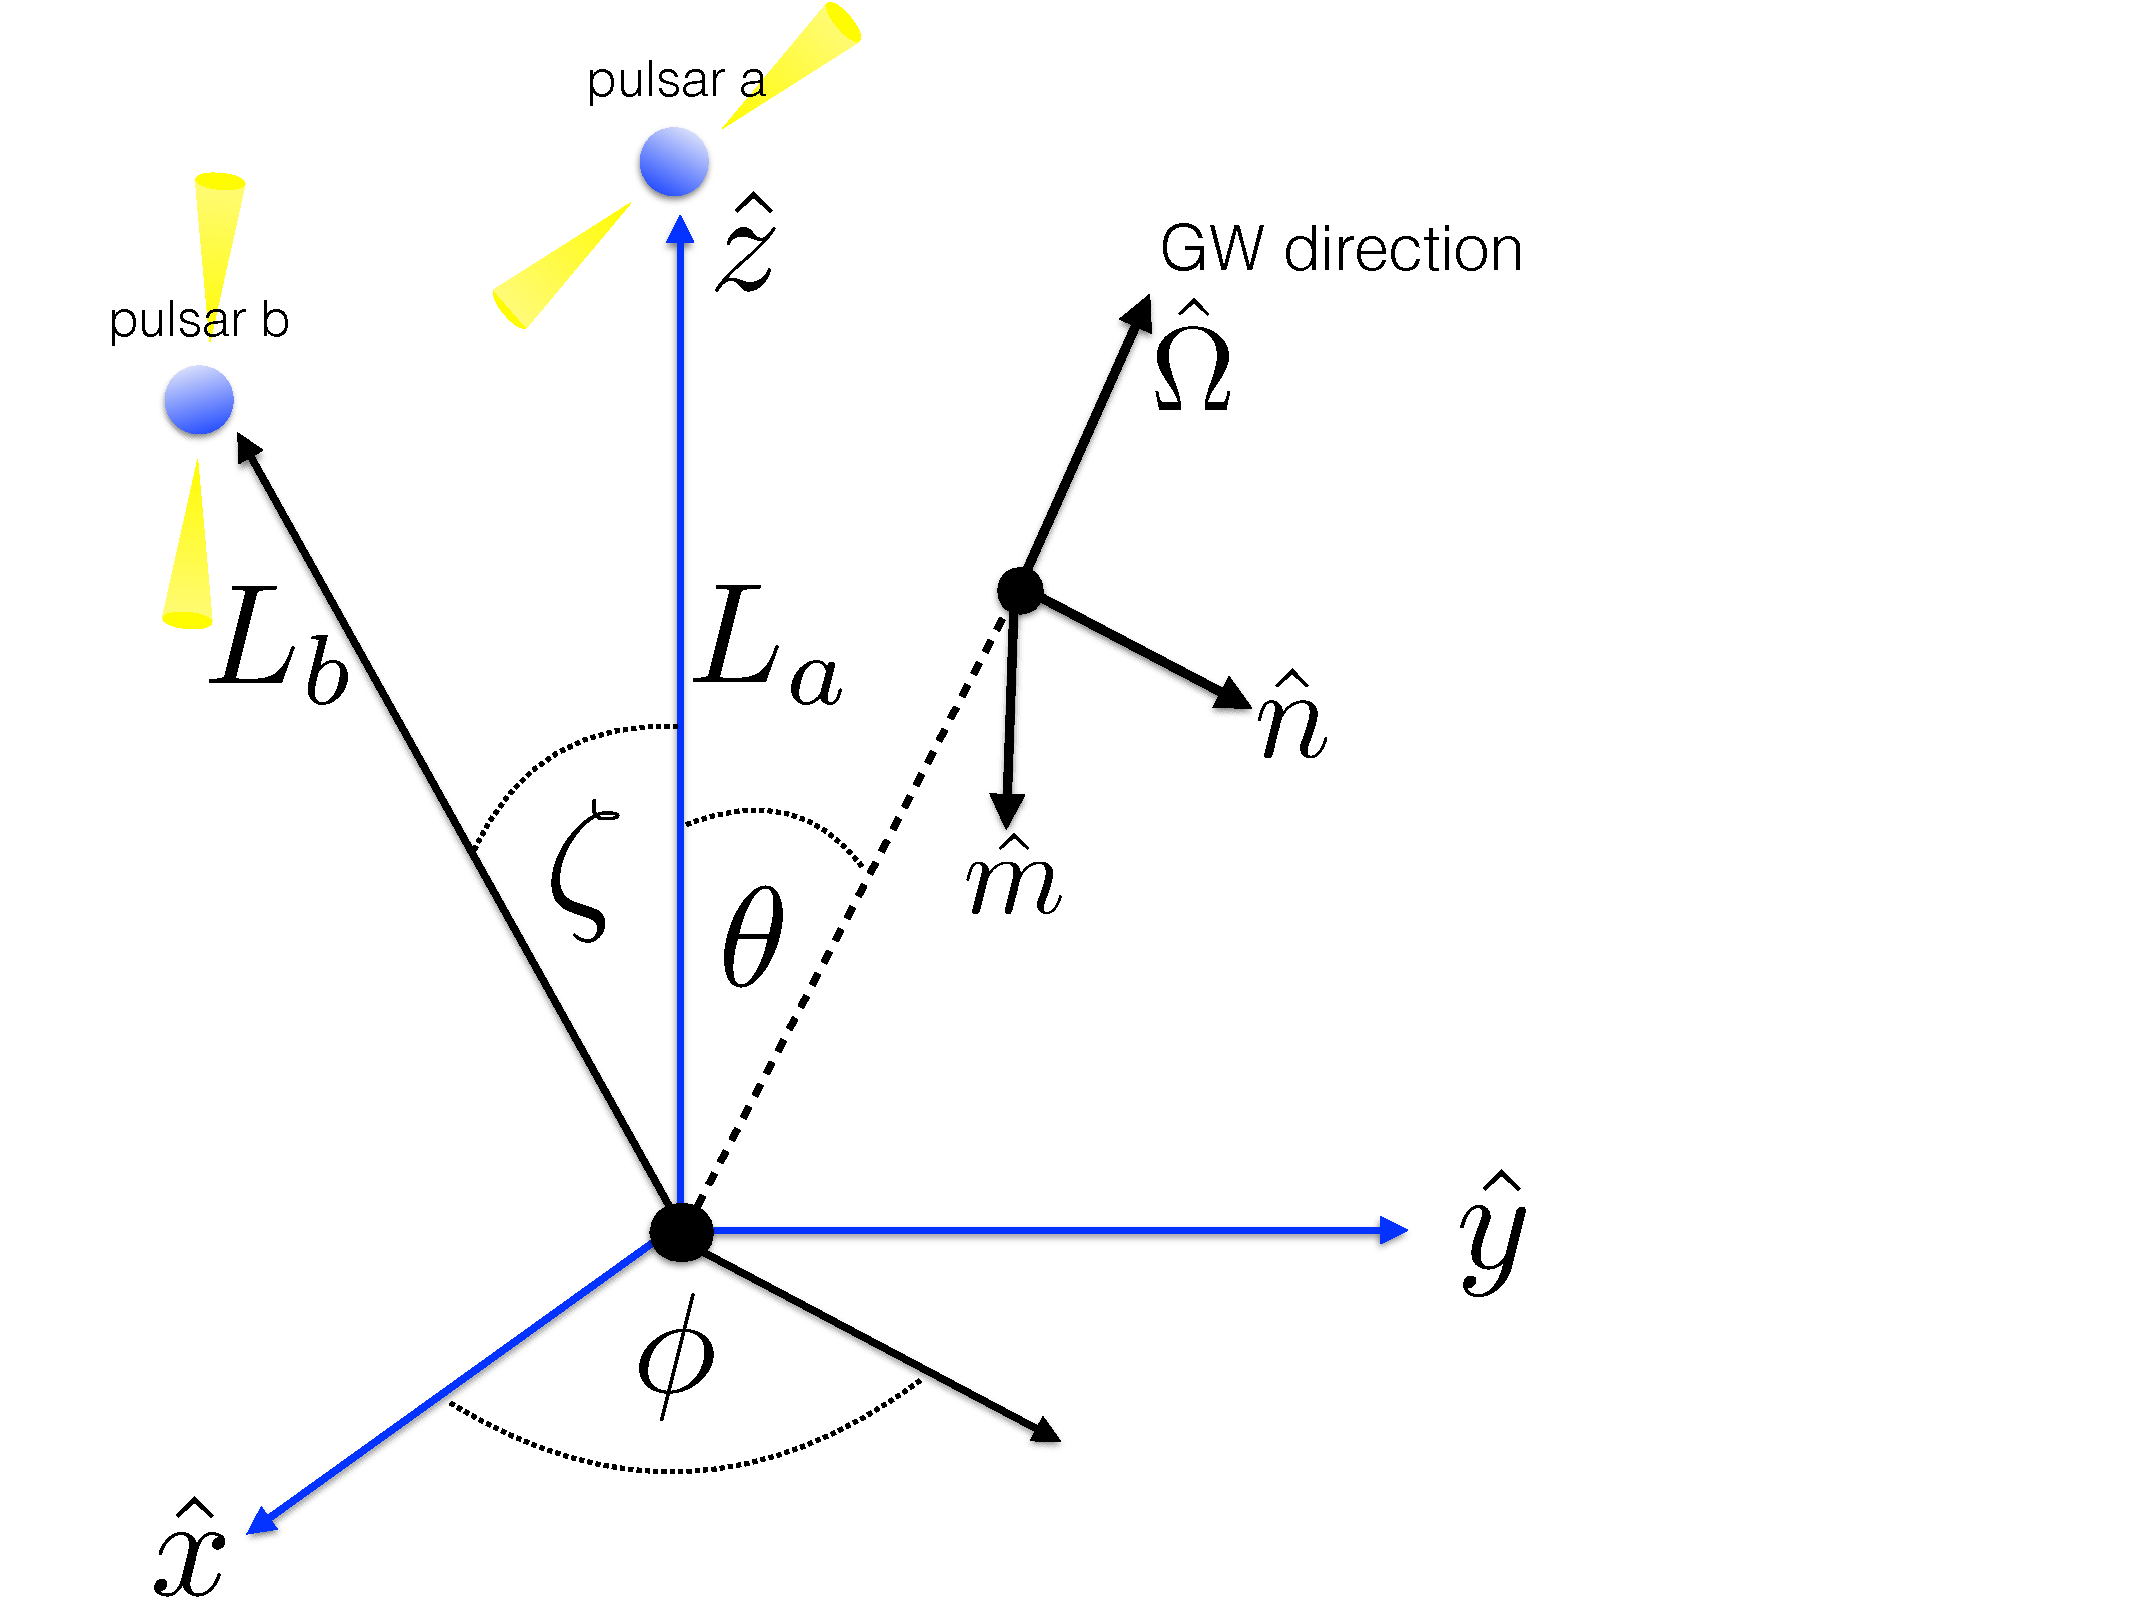
\includegraphics[width=3.9in]{pta_geometry.pdf}
		\caption[Typical pulsar timing array geometry]{Suggested geometry: pulsar $a$ is on the $z$-axis at a distance $L_a$ from the origin (solar system barycentre), pulsar $b$ is in the $x$-$z$ plane at a distance $L_b$ from the origin making an angle $\zeta$ with pulsar $a$. $\hat\Omega$ is the direction of GW propagation with principal axes $\hat m$ and $\hat n$ such that  $\hat m \times \hat n =\hat\Omega$. The polar and azimuthal angles are given by $\theta$ and $\phi$, respectively.}
		\label{fig:geometry}
	\end{figure}
\item Write down the general expression for the antenna beam pattern, 
\begin{equation}
F^A(\hat \Omega) = \frac{1}{2} \frac{\hat p^i \hat p^j}{1+\hat\Omega\cdot\hat p} e^A_{ij}(\hat\Omega) \, ,  
\end{equation}
where $A=+,\times$ is the GW polarization. The polarization tensors $e^+_{ij}(\hat \Omega) = \hat m_i\hat m_j - \hat n_i \hat n_j$, $e^\times_{ij} (\hat \Omega)= \hat m_i \hat n_j + \hat n_i \hat m_j$. For further reading, see \cite{AllenRomano:1999, Anholm:09}. 


[Solution]
\begin{subequations}
\begin{align}
F^+_a &= \frac{1}{2} \frac{(\hat m \cdot \hat p_a)^2-(\hat n \cdot \hat p_a)^2}{1+\hat\Omega\cdot\hat p_a}\, ,\\
F^\times_a &= \frac{(\hat m \cdot \hat p_a)(\hat n \cdot \hat p_a)}{1+\hat\Omega\cdot\hat p_a}\, .
\end{align}
\end{subequations}

\item Give expressions for $F^+_a$, $F^\times_a$, $F^+_b$, $F^\times_b$ in your chosen coordinate frame.

[Solution]
In the reference frame given in Fig \ref{fig:geometry}, one can now write down the antenna beam patterns as follows:
\begin{subequations}
	\label{e:F+Fx_comp}
	\begin{align}
	&F^\times_a=0,\\ 	
	& F^+_a=-\frac{1}{2}(1-\cos\theta),\\
	&F^\times_b\!\!=\! \!\frac{(\sin\phi\,\sin\zeta\!)(\cos\theta\!\sin\zeta\!\cos\phi\!-\!\sin\theta\!\cos\zeta\!)}{1\!+\!\cos\theta\!\cos\zeta+\sin\theta\!\sin\zeta\cos\phi},\\
	&F^+_b\!\!=\!\!\frac{1}{2}\frac{(\sin\phi\sin\zeta\!)^2\!\!-\!(\sin\zeta\!\cos\theta\!\cos\phi-\sin\theta\!\cos\zeta\!)^2}{\!1\!+\!\cos\theta\cos\zeta+\sin\theta\sin\zeta\cos\phi}.\nonumber\\
	\end{align}
\end{subequations}
This choice of geometry is commonly refereed to as the ``computational frame'', since here $F_a^\times = 0$, greatly simplifying analytical calculations to follow.
	
\item The overlap reduction function is given by integrating the antenna beam patterns over the sky, i.e. over all possible GW directions $\hat \Omega$:
\begin{equation}
\label{eq:ORF}
^{(ab)}\Gamma(\zeta)=\int_0^\pi  \sin\theta d\theta \int_0^{2\pi} d\phi  \sum_A F^A_a(\hat \Omega) F^A_b(\hat \Omega) \, ,
\end{equation}
where $\zeta \in [0,\pi] $ is the angle between the pulsars. Using your expressions for the antenna beam pattern, you may either integrate the above expression analytically (hint, use contour integration) or open the ipython notebook and do this numerically. Plot the result for all $\zeta$. The result is the Hellings and Downs curve! 


[Analytical Solution]

Substituting Eq.~(\ref{e:F+Fx_comp}) into Eq.~(\ref{eq:ORF}), the overlap reduction functions become:
\begin{equation}
	{}^{(ab)}\Gamma(\zeta) \! = \!-\frac{1}{4}\int_0^\pi \!\!\!d\theta\sin\theta \!\! \int_0^{2\pi}\!\!\!\!d\phi
	\frac{(1-\cos\theta)(\sin^2\zeta\sin^2\phi-\sin^2\zeta\cos^2\theta\cos^2\phi-\cos^2\!\zeta\sin^2\theta+2\sin\zeta\!\cos\zeta\!\sin\theta\cos\theta\cos\phi )}
	{1+\sin\zeta\sin\theta\cos\phi+\cos\zeta\cos\theta}\, .
	\label{e:Gammalm_ex}
\end{equation}
One can write Eq \eqref{e:Gammalm_ex} as the sum of two integrals: 

\begin{equation}
^{(ab)}\Gamma=\frac{1}{4}(Q+R)\label{eq:quarterGamma}\, , 
\end{equation}

where
\begin{eqnarray}
Q &=&  \int_0^\pi \!\!d\theta\sin\theta(1\!-\!\cos\theta) \int_0^{2\pi}d\phi (1\!-\!\cos\zeta\!\cos\theta\!-\!\sin\zeta\!\sin\theta\cos\phi)\\
&=&\sqrt{4\pi}\left(1+\frac{\cos\zeta}{3}\right).
\label{eq:AppQ}
\end{eqnarray}
and
\begin{eqnarray}
	&&R\!=\!\!-2\sin^2\zeta\!\!\int_0^{\pi}\!\!\!d\theta\sin\theta(1\!-\!\cos\theta)I \label{eq:appendixRLM}  \\
	&&I\equiv\!\!\int_0^{2\pi}\!\!\!d\phi\frac{\sin^2\phi}{1+\cos\zeta\!\cos\theta+\sin\zeta\!\sin\theta\cos\phi}\, .
	\label{eq:Im}
\end{eqnarray}
Eq \eqref{eq:Im} is evaluated via contour integration (or via Maple/Mathematica, whatever you like!)

\begin{eqnarray}
I&=&2\pi\frac{1+\cos\zeta\cos\theta-|\cos\zeta+\cos\theta|}{\sin^2\zeta\sin^2\theta}\label{eq:An1}\\
I&=&2\pi
 \left\{
\begin{array}{lc}
\left(\frac{1-\cos\zeta}{\sin^2\zeta}\right)\left(\frac{1-\cos\theta}{\sin^2\theta}\right), &		 	0<\theta<\pi-\zeta 	\\
\left(\frac{1+\cos\zeta}{\sin^2\zeta}\right)\left(\frac{1+\cos\theta}{\sin^2\theta}\right), &	 \pi-\zeta<\theta<\pi \label{eq:R00pm}\\
\end{array}
\right.
\end{eqnarray}

We can now write down the final form of $R$:
\bea
R&=&-\frac{4\pi(1-\cos\zeta)}{\sqrt{4\pi}}\!\int_0^{\pi-\zeta}\!\!\! d\theta  \frac{(1-\cos\theta)^2}{\sin\theta}-\frac{4\pi(1+\cos\zeta)}{\sqrt{4\pi}}\!\int_{\pi-\zeta}^\pi\!\!\! d\theta\sin\theta\\
&=&\sqrt{4\pi}(1-\cos\zeta)4\ln\left(\sin\frac{\zeta}{2}\right).
\eea

 Using Eq \eqref{eq:quarterGamma}, one may write the isotropic solution to Eq \eqref{e:Gammalm_ex}:
\begin{equation}
{}^{(ab)}\Gamma(\zeta)=\frac{\sqrt{\pi}}{2}\left[1+\frac{\cos\zeta}{3}+4\beta\ln\left(\sin\frac{\zeta}{2}\right)\right]\, .
\end{equation}
This equation is the Hellings and Downs curve up to a multiplicative factor.

\item Normalize this curve such that when $\zeta=0$, $^{(ab)}\Gamma(\zeta)=0.5$. What is this normalization factor?

$4\sqrt{\pi}/3$. In fact the Hellings and Downs curve is normalized such that it is equal to 1 for  $\zeta = 0$, {\it i.e.} pulsar $a =$ pulsar $b$, but that discussion is beyond the scope of this course. If you're interested in knowing more about this, see \cite{MingarelliSidery:2014}.


\item Which of these steps implicitly assumes an isotropic background? Where would we modify this calculation to take in to account anisotropy in the GW background? More on this in \cite{MingarelliEtAl:2013}.

In the evaluation of the overlap reduction function, one can add an angular power distribution, $P(\hat\Omega)=\sum_{lm}c_{lm}Y_{lm}$, which then allows for anisotropy. The $Y_{lm}$ are the regular spherical harmonics.
\end{enumerate}







\bibliography{references}





\end{document}